\subsection{Model Evaluation}
\label{sec:evaluation}

To evaluate the new model,
we implemented a power estimator consisting of
a sampling-based frame recorder
by modifying the Android screenrecord command code,
and a power calculator that implements Steps 2--4 in a C++ program with ~1 KLOC.
% using OpenCV Library.
It takes a pixel sampling ratio and the phone
display power model as input, records a frame,
and outputs the estimated display power consumption.
Below, we evaluate the accuracy and runtime of the
power estimator 
% running on the three phones
and how sampling affects their tradeoff.

% \subsection{Model Evaluation}

\if 0
We calculated the prediction error of the new model
in predicting the power at the center point of each color cube.
Using measured and estimated current, we calculated the error value.
The average error using linear and non-linear model was found to be less
than 5\%. For Nexus 6 , the average error is  3\% both both models. For Pixel 2,
average error was 2\% and 3\% for linear and non-linear model respectively.

We concluded from the above findings that linear model is good to use for
estimation,though non-linear model can provide us marginally better estimation.
This is because though the error is small in non linear model 
and the computation requirement in linear model is quite less in comparison
to non-linear model.
\fi


% \subsection{Accuracy}

\paragraph{Methodology.}
%  We evaluate the accuracy of the new pixel power model following the
%  same methodology as in \S\ref{sec:measurement}, \ie displaying static
%  images one at a time, recording the OLED display power reading from the
%  power sensor, and comparing the model estimated power against the
%  ground truth.
% We evaluate the accuracy of the new pixel power model with a set of 100
% images taken from Google Images, comprising both digitally generated and
% natural images. The set of images covers 10 diverse categories of content:
% Abstract, Animals, Birds and Fish,
% Cartoon, 3D CGI, Flower, Painting,
% Landscape, Plain, Fruits/Vegetables, and Mountains/Rivers.
% We evaluate the accuracy of the new pixel power model with a set of 100
% images taken from Google Images, comprising both digitally generated and
% natural images.
We evaluate the accuracy of the new pixel power model with a set of screenshots
 for 5 activities each for 6 popular Google apps,
Calculator, Calendar, Maps, Phone, News, and YouTube,
under both dark and light modes.
We measure the ground truth OLED power
following the same methodology as in \S\ref{sec:measurement}.
\forjnl{as shown in Figure~\ref{fig:100_images_expriment}.}
% including Abstract, Animals, Birds \& Fish, Cartoon, 3D CGI, Flower,
% Painting, Landscape, Plain, Fruits \& Vegetables, and Mountains \& Rivers.
To evaluate the impact of pixel sampling, we vary the sampling ratio
from 1 (no sampling) to 4096.
% The runtime of model application was measured on a Windows laptop.

% We want to evaluate the OLED current model with running our app. The limitation being
% that there can be various other current consuming components in the mobile phone
% like CPU, GPU to state a few and these are also required to be accurately
% modelled to extract a very accurate OLED screen power. We considered a middle path
% and decided to use an Android app ExoPlayer which has a very low overhead , so that
% we can extract the OLED display current more accurately.


\paragraph{Impact of subgrid size.}
We first measure the prediction error of P-LMLR and P-NLM models across
% the 100 images
the activity screenshots from the 6 Google apps
under subgrid sizes 16 and 32, on the three phones, respectively.
The results show that using subgrid sizes 16 and 32 result in very similar
prediction errors.  Since using subgrid size
16 only needs 64KB 
to store the 4096 piecewise models (of 4 coefficients each),
which is insignificant, and incurs
negligible application time (see below),
but can better cope with potential OLED power fluctuations (\eg on other phones),
% from being able to fit the piecewise models
% in the L2 cache when processing on a laptop.
we use subgrid size $16\times 16\times 16$ in our model design.

\if 0
\begin{figure*}[th]
	\begin{subfigure}[]{0.29\textwidth}
		\includegraphics[width=\textwidth]{./figure/700_100Image_N6_Standard.pdf}
		\caption{Nexus 6}
	\end{subfigure}
	\hfill
	\begin{subfigure}[]{0.29\textwidth}
		\includegraphics[width=\textwidth]{./figure/703_100Image_P2_Boosted.pdf}
		\caption{Pixel 2}
	\end{subfigure}
	\hfill
	\begin{subfigure}[]{0.29\textwidth}
		\includegraphics[width=\textwidth]{./figure/701_100Image_Z3_Vibrant.pdf}
		\caption{Moto Z3}
	\end{subfigure}
        \vspace{-0.1in}
	\caption{Measured and predicted OLED power draw using P-LMLR
          for 100 images in 10 categories (A: Abstract, B: Animals, Birds and Fish,
			C: Cartoon, D: 3D CGI, E: Flower, F: Painting, G: Landscape, H: Plain,
			I: Fruits / Vegetables, J: Mountains / Rivers).}
	\label{fig:100_images_expriment}
\end{figure*}
\fi


\paragraph{Impact of sampling ratio.}
Figure~\ref{fig:smapling_error} left shows the additional
prediction error of P-LMLR when increasing the pixel sampling ratio
compared to that of P-LMLR without sampling,
for the set of activity screenshots from the 6 Google apps on the 3 phones.
% The error here is calculated w.r.t. to the current estimated with no sampling as base value.
We see that increasing the sampling ratio increases the prediction error
slowly. The additional error predicted is less than 1\% for the
3 phones at the sampling ratio of 100.

% \begin{figure}[tp]
% 	\begin{subfigure}[]{\columnwidth}
% 		\includegraphics[width=0.48\columnwidth]{./figure/501_N6_error.pdf}
%  		\includegraphics[width=0.48\columnwidth]{./figure/502_N6_time.pdf}
% 		\caption{Nexus 6}
% 	\end{subfigure}
% 	
% 	\begin{subfigure}[]{\columnwidth}
% 		\includegraphics[width=0.48\columnwidth]{./figure/503_P2_error.pdf}
%  		\includegraphics[width=0.48\columnwidth]{./figure/504_P2_time.pdf}
% 		\caption{Pixel 2}
% 	\end{subfigure}
% 	\begin{subfigure}[]{\columnwidth}
% 		\includegraphics[width=0.48\columnwidth]{./figure/505_Z3_error.pdf}
%  		\includegraphics[width=0.48\columnwidth]{./figure/506_Z3_time.pdf}
% 		\caption{Moto Z3}
% 	\end{subfigure}
%         \vspace{-0.1in}
% 	\caption{Prediction error of and runtime in applying the P-LMLR model under various
%           sampling ratios.}
%        \vspace{-0.1in}
% 	\label{fig:smapling_error}
%        \vspace{-0.1in}
% \end{figure}

% \begin{figure}[tp]
% 	\begin{subfigure}[]{\columnwidth}
% 		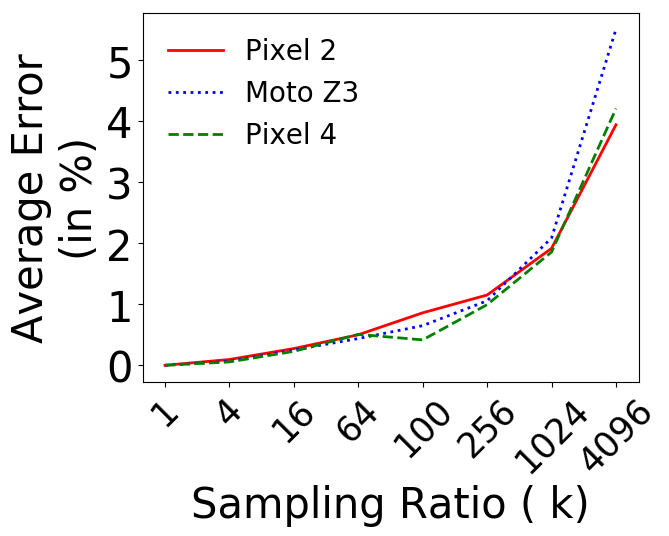
\includegraphics[width=0.48\columnwidth]{figure/001_sampling_ratio_error.png}
%  		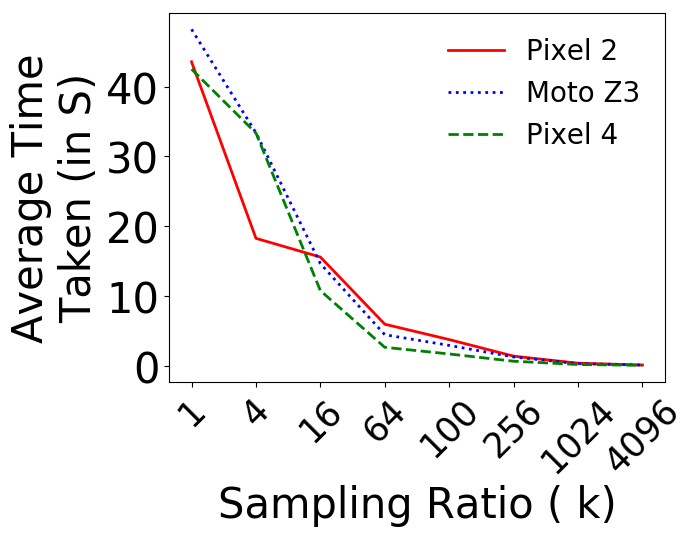
\includegraphics[width=0.48\columnwidth]{figure/002_sampling_ratio_time.png}
% 	\end{subfigure}
%         \vspace{-0.1in}
% 	\caption{Prediction error of and runtime in applying the P-LMLR model under various
%           sampling ratios.}
%       \vspace{-0.1in}
% 	\label{fig:smapling_error}
%     %\vspace{-0.1in}
% \end{figure}

\begin{figure}[tp]
	\begin{subfigure}[]{0.48\columnwidth}
		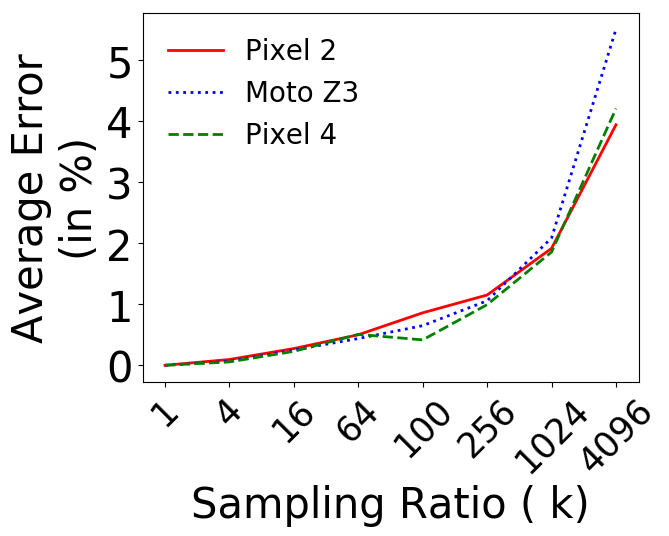
\includegraphics[width=\columnwidth]{figure/001_sampling_ratio_error.png}
		\caption{Additional model error}
		\label{fig:eval_smapling_error_error}
	\end{subfigure}
	\begin{subfigure}[]{0.48\columnwidth}
 		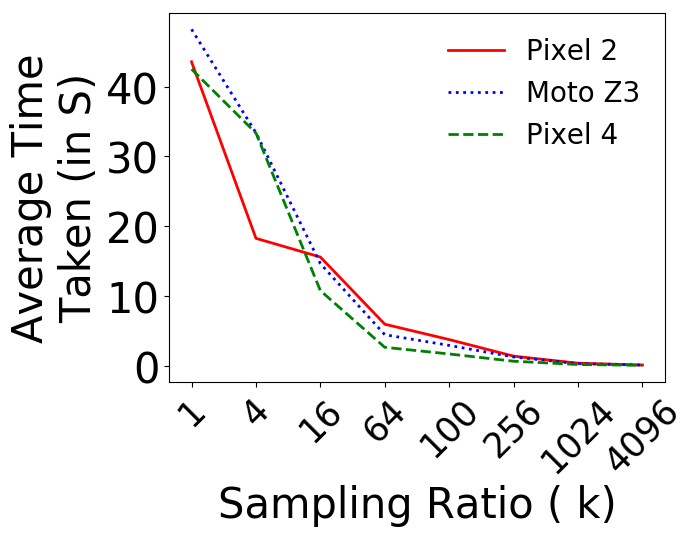
\includegraphics[width=\columnwidth]{figure/002_sampling_ratio_time.png}
 		\caption{Average runtime (T1+T2)}
 		\label{fig:eval_smapling_error_time}
	\end{subfigure}
	\vspace{-0.1in}
	\caption{Additional prediction error of and runtime in applying the P-LMLR model under various
          sampling ratios.}
	\label{fig:smapling_error}
    \vspace{-0.1in}
\end{figure}

%% This for the phone results. Above is the computer results
% \begin{figure}[tp]
% 	\begin{subfigure}[]{\columnwidth}
% 		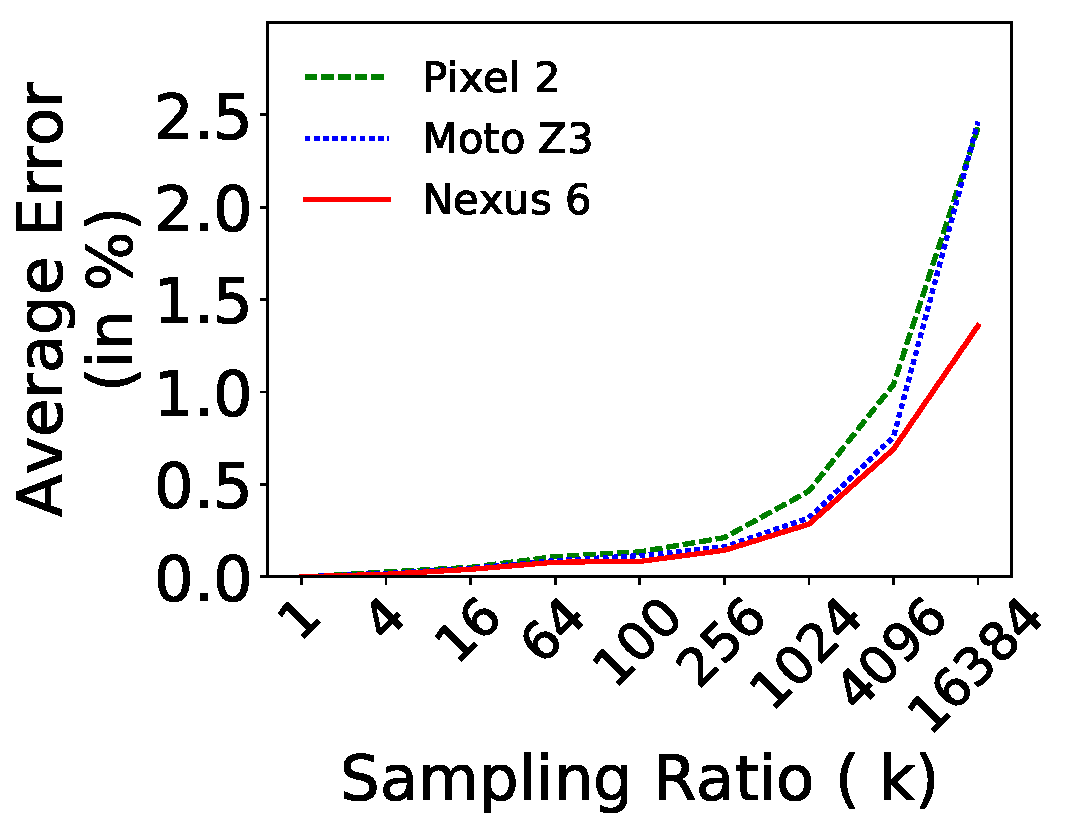
\includegraphics[width=0.48\columnwidth]{./figure/511_All_error.pdf}
%  		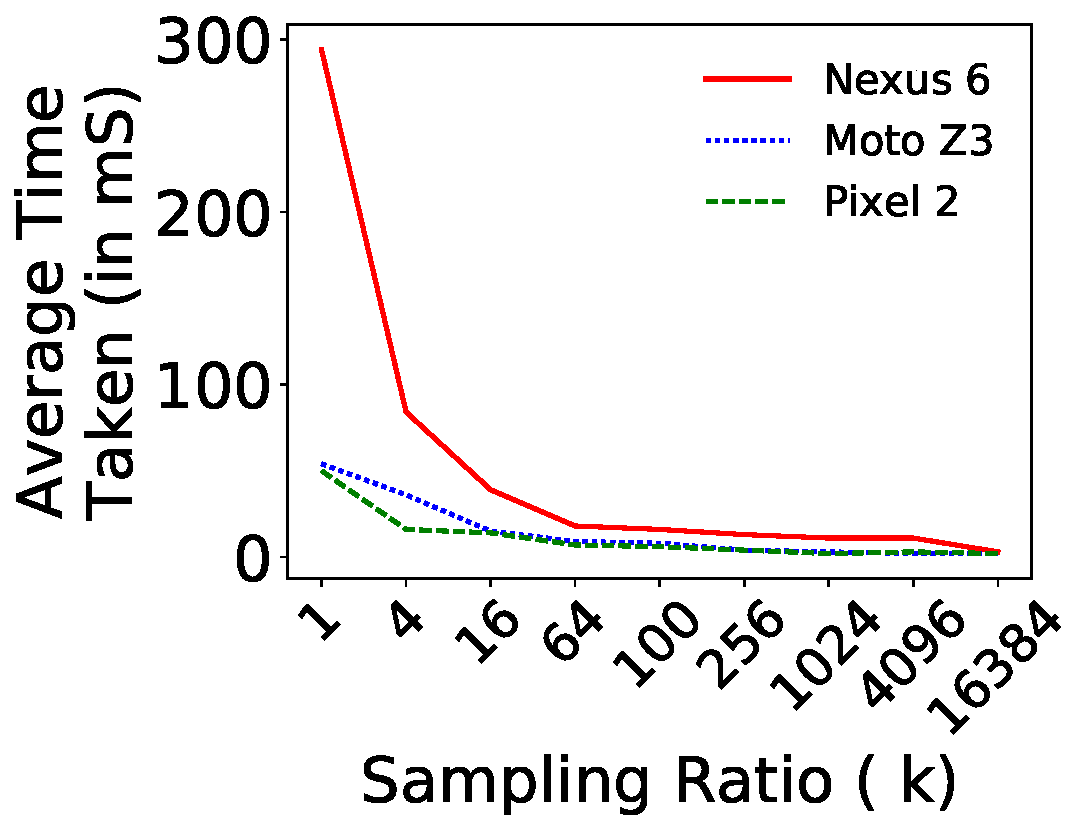
\includegraphics[width=0.48\columnwidth]{./figure/511b_All_time.pdf}
% 	\end{subfigure}
%         \vspace{-0.1in}
% 	\caption{Prediction error of and runtime in applying the P-LMLR model under various
%           sampling ratios.}
%        \vspace{-0.1in}
% 	\label{fig:smapling_error}
%        \vspace{-0.1in}
% \end{figure}

% \subsection{Model Application Runtime}

%  \paragraph{Methodology}
%  Further our Power model c++ program also generate the runtime overhead
%  incurred at various sampling ratios for the 100 images. 
%  As mentioned earlier, we used the sampling ratio from 0.01 \% to 90 \% and
%  %  ran this experiments on the server and during this we measured run time over heads. \dcomment{Get Specs}

\paragraph{Frame recording and power calculation time.}
Figure~\ref{fig:smapling_error} right shows how the sampling
ratio affects the total time (frame recording time (T1) 
plus power calculation
time (T2)) in applying the P-LMLR model to
calculate the power for a given frame.
%   {
%   This contains the frame capture and model application overhead.
%   Without sampling, the computation takes 8.3 ms, 4.4 ms and 4.1 ms on
%   the 3 phones which less than 10\% on the total time taken.
%   }
We observe that for all three
phones, the total time and two individual times not shown are inversely proportional to the
sampling ratio. In particular, without sampling, the frame recording
time are 10ms, 10ms, and 4ms
and
the power calculation time are 44ms, 48ms and 42ms on
 the three phones,
while with a sampling ratio of 100, the recording time are reduced to
1ms, 1ms, and 1ms, and power calculation time are reduced to
4ms, 3ms, and 2ms, respectively.
We note the long frame recording time is due to the delay in pulling data from frame buffer
and does not keep CPU busy.
As we will show in \S\ref{subsec:tool2},
the average CPU utilization of power calculation
is only 1.1\%, 0.9\%, and 0.6\% on Pixel 2, Moto Z3, and Pixel 4, respectively.
\if 0
The reduced model application runtime allows the OLED display power to
be calculated for a recorded app run (one frame every 16.7ms at 60
FPS) at less than 1/10th of the app run duration, in
post-processing.
\fi
We thus conclude that a sampling ratio of 100 strikes
a good balance between minimal prediction accuracy loss and sufficient
model application runtime reduction.

% \begin{figure}[]
% 	\includegraphics[width=\columnwidth]{./figure/401_Model_Compariosn.png}
% 	\caption{The heat map of the display current shows the different in the OLED
% 		model between the two generatios of the OLED display technology}
% 	\label{fig:oled_model_comparison}
% \end{figure}

% \begin{figure*}[tp]
% 	\begin{subfigure}[]{0.33\textwidth}
% 		\includegraphics[width=\textwidth]{./figure/200_n6_simple.pdf}
% 		\caption{Nexus 6}
% 	\end{subfigure}
% 	\begin{subfigure}[]{0.33\textwidth}
% 		\includegraphics[width=\textwidth]{./figure/201_z3_vibrant.pdf}
% 		\caption{Moto Z3 Neutral Standard Color Mode}
% 	\end{subfigure}
% 	\begin{subfigure}[]{0.33\textwidth}
% 		\includegraphics[width=\textwidth]{./figure/201_z3_vibrant.pdf}
% 		\caption{Moto Z3 Neutral Vibrant Color Mode}
% 	\end{subfigure}
% 	\hfill
% 
% 	\centering
% 	\begin{subfigure}[]{0.33\textwidth}
% 		\includegraphics[width=\textwidth]{./figure/203_p2_boosted.pdf}
% 		\caption{Pixel 2 Boosted Color Mode}
% 	\end{subfigure}
% 	\begin{subfigure}[]{0.33\textwidth}
% 		\includegraphics[width=\textwidth]{./figure/204_p2_natural.pdf}
% 		\caption{Pixel 2 Natural Color Mode}
% 	\end{subfigure}
% 	\begin{subfigure}[]{0.33\textwidth}
% 		\includegraphics[width=\textwidth]{./figure/205_p2_staturated.pdf}
% 		\caption{Pixel 2 Saturated Color Mode}
% 	\end{subfigure}
% 
% 	\caption{The current consumed by the OLED display with varying RGB values
%         on three phones, Nexus 6, Moto Z3 Plus (2 color modes), and Pixel 2 (3 color modes).}
% 	\label{fig:initial_evaluation}
% \end{figure*}

% \begin{figure}[!htb]
% 	\centering
% 	\begin{tabular}[t]{|c|c|}
% 	\hline
% 	
%     \begin{subfigure}{0.4\textwidth}
%     \centering
%     \smallskip
%     \includegraphics[width=0.9\linewidth,height=1.7\textwidth]{./figure/904_Current_Model_Comparision.png}
%     \caption{Cat 1} %{Light Unit}
% \end{subfigure}
%     &
%         \begin{tabular}{c}% if you add [t], than sub images are pushed down
%         \smallskip
%             \begin{subfigure}[t]{0.4\textwidth}
%                 \centering
%                 \includegraphics[width=0.9\textwidth]{./figure/900_BASE_Model_Comparision.png}
%                 \caption{Cat 2}
%             \end{subfigure}\\
%             \begin{subfigure}[t]{0.4\textwidth}
%                 \centering
%                 \includegraphics[width=0.9\textwidth]{./figure/903_P2_Model_Comparision.png}
%                 \caption{Cat 3}
%             \end{subfigure}
%         \end{tabular}\\
% \hline
%     \end{tabular}
%     \caption{Cats}
% \end{figure}

% \begin{table}[h]
% \begin{center}
% 	\centering
% 	\caption{Popular Google Android App Experiment Methodology}
% 	\begin{tabular*}{\columnwidth}{@{\extracolsep{\fill}}| l | l | r |}
% 		\hline
% 		Phone        & Average Error & Average Time\\
% 		\hline
% 		Nexus 6      & .06 \%        & 11 \\
% 		Moto Z3      &  2.9 \%        & 11 \\
% 		Pixel 2      & 	1.7 \%        & 11 \\
% 		\hline
% 	\end{tabular*}
% 	\label{tab:100_images}
% \end{center}
% \end{table}


% \begin{table}[tp]
% \begin{center}
% \centering
% \caption{Mean (median) display power prediction error for the 6 app activity screenshots.}
% %  (50 percentile | 90 percentile)
% % \dcomment{Showing both numbers. Not to be included in final}
% \vspace{-0.1in}
% \footnotesize
% % \begin{tabular*}{\columnwidth}{ | p{0.12\columnwidth} | p{0.20\columnwidth} | p{0.20\columnwidth} | p{0.20\columnwidth} | p{0.20\columnwidth}  }
% \begin{tabular*}{\columnwidth}{@{\extracolsep{\fill}}|p{10mm}|c|c|c|c|c|}
% 	\hline
% 	       \multirow{2}{*}{Phone} & \multirow{2}{*}{Mode} & \multicolumn{4}{c|}{Average Percentage Error} \\
% 	\cline{3-6}
% 	        &   & LMLR & NLM & P-LMLR & P-NLM\\
% 	\hline
% 	{Pixel } & dark   & 21.6 ( 23.3) & 12.8 ( 13.5) & 4.2 ( 3.9) & 3.5 ( 2.3) \\
% 	                         % \cline{2-6}
% 	       2                  & light  & 7.2 ( 7.5) & 5.4 ( 5.5) & 1.7 ( 1.5) & 1.7 ( 1.5) \\
% 	\hline
% 	{Moto } & dark   & 17.3 ( 20.1) & 11.8 ( 13.7) & 3.1 ( 3.1) & 3.5 ( 3.6) \\
% 	                         % \cline{2-6}
% Z3	                         & light  & 5.0 ( 5.6) & 4.8 ( 5.5) & 2.2 ( 2.0) & 2.3 ( 2.1) \\
% 	\hline
%     {Pixel } & dark   & 18.9 ( 17.0) & 13.1 ( 11.8) & 4.3 ( 4.5) & 4.6 ( 4.6) \\
%                              % \cline{2-6}
%           4                  & light  & 6.5 ( 7.4) & 7.5 ( 7.9) & 2.6 ( 1.0) & 2.7 ( 0.9) \\
% 	\hline
% \end{tabular*}
% \label{tab:100_images}
% \end{center}
% \vspace{-0.15in}
% \end{table}

\begin{table}[tp]
\begin{center}
\centering
\caption{Mean (median) display power prediction error for the 6 app activity screenshots.}
\vspace{-0.1in}
{ \footnotesize
    \begin{tabular}{|p{7mm}|p{6mm}|c|c|c|c|}
    	\hline
    	       \multirow{2}{*}{Phone} & \multirow{2}{*}{Mode} & \multicolumn{4}{c|}{Average Percentage Error} \\
    	\cline{3-6}
    	        &   & LMLR & NLM & P-LMLR & P-NLM\\
    	\hline
    	Pixel & dark   & 21.6 (23.3) & 12.8 (13.5) & 4.2 (3.9) & 3.5 (2.3) \\ % \cline{2-6}
    	    2 & light  & 7.2 (7.5) & 5.4 (5.5) & 1.7 (1.5) & 1.7 (1.5) \\
    	\hline
    	Moto  & dark   & 18.9 (17.0) & 13.1 (11.8) & 4.3 (4.5) & 4.6 (4.6) \\ % \cline{2-6}
           Z3 & light  & 6.5 (7.4) & 7.5 (7.9) & 2.6 (1.0) & 2.7 (0.9) \\
    	\hline
        Pixel & dark   & 17.3 (20.1) & 11.8 (13.7) & 3.1 (3.1) & 3.5 (3.6) \\ % \cline{2-6}
            4 & light  & 5.0 (5.6) & 4.8 (5.5) & 2.2 (2.0) & 2.3 (2.1) \\
    	\hline
    \end{tabular}
}
\label{tab:100_images}
\end{center}
\vspace{-0.2in}
\end{table}
% \footnotetext{The error depends on the images tested as it is content specific.}

\paragraph{Accuracy.}
\forjnl{Figure~\ref{fig:100_images_expriment} shows the measured and predicted
OLED power draw using the new piecewise linear model (P-LMLR) for the
100 images and the prediction error for each on the three phones. We
see that using P-LMLR, the estimated OLED display power closely follows
the measured power for all 3 phones.}
Table~\ref{tab:100_images}
summarizes the average prediction error by LMR, NLM, P-LMLR, and P-NLM
for the activity screenshots with 100x sampling on the three phones.
The error for LMLR and NLM varies across the phones,
because their error for individual pixel colors vary in different regions of the color space
on different phones (Figure~\ref{fig:initial_evaluation_2})
and different images have different distribution of pixel colors.
In contrast, the prediction errors of P-NLM and P-LMLR are
almost identical and consistent across the 3 phones,
\ie the two models are robust to phone diversities,
% (within 10\%),
and the errors are significantly lower than that of LMLR and NLM.
In particular, P-LMLR reduces the average prediction error
of LMLR by
    5.1$\times$, 5.5$\times$ and 4.4$\times$ for dark mode
    and 4.2$\times$, 2.3$\times$ and 2.5$\times$ for light mode for the three phones.
%     \nexuserrorreduction,
%     \pixelerrorreduction, and
%     \motoerrorreduction,
%     from
%     \nexuserror, \pixelerror, and \motoerror
% down to 3.3\%, 3.3\%, and 2.9\% on the 3 phones.

% \dcomment{Add this}
% We recorded the screen from various apps and play it on the Android app and
% compared to the ground truth. We used a CPU and GPU model \dcomment{cite}
% to find the accuracy of the OLED model to be .

